\section{Brainstorm}
\label{brainstorm}

\paragraph{The execution}
Brainstorming is not an exact science, therefore there is no pre-defined schema to follow.
However, there are a lot of gurus describing guidelines to manage sessions.
The following list is an implementation of guidelines taken from Tyner Blain \cite{brainstormWebsite}:

\begin{enumerate}
	\item \textbf{Rules -} Make sure everyone is on the same level and understands what the point of the meeting is.
	\item \textbf{Time limit -} Guidelines describe short sessions, but the complexity of the system meant that two sessions of one hour each were necessary.
		The next step (seed) was repeated in the second session to refresh the idea of the system for everyone.
	\item \textbf{Seed -} A starting point is needed, in this case an educated guess is used.
		The system seed is described in \ref{process-analysis}.
		During the session big (A2) pieces of paper are used on which the seed's functions are written down, figure \ref{fig:brainstorm-before} is a stylised version of this paper schema.
	\item \textbf{Ideas -} The sessions are structured by the paper schema, each of the functions is discussed.
		Ideas for new functionality or differences are shortly (vocally) summarised by the session leader and written on the same paper.
	\item \textbf{Prioritise -} For this step the guidelines are disregarded, prioritisation is based on group agreement.
		Three levels are used: must have, should have, nice to have.
		Any functions that are deemed unnecessary were already removed from the schema during the previous step.
\end{enumerate}

\paragraph{Results: differences and similarities}
Outcomes of the brainstorm showed that a lot of functions were initially hidden when the system seed was defined.
Next to data management there were also user, publication, and (more extensive) request management requirements.
In the sense of the research workflow schema not much has changed visually, publication and user groups are added.
The publication functions support the last phase in research and the user functions underlay the whole system.

\begin{figure}[hb]
	\centering
	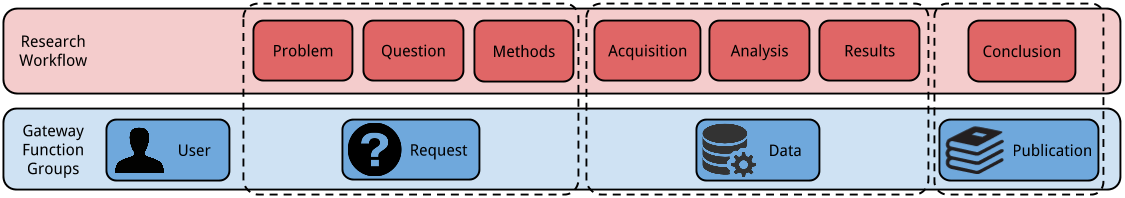
\includegraphics[width=1.0\linewidth]{images/research-workflow-after}
	\caption{
		Research workflow mapped by identified function groups after brainstorm, initial workflow shown in figure \ref{fig:research-workflow}.
		The user group underlays the whole system and is therefore outside of the dotted mapping lines.
	}
	\label{fig:workflow-after}
\end{figure}

When looking at the expanded view (figure \ref{fig:brainstorm-after}) however a lot more changes are visible.
In the external parts (services and users) some changes took place.
Unlinked data has been removed from the input as it has no scientific value in the type of research that the system is going to support.
This is because unlinked means that either no treatment was found for a particular birth or no birth was found for a treatment.
Analysis on correlations in these groups (\ie{} \emph{why} could no link be found) might be interesting but are currently outside of the scope of the \project{}.

External parties and principal investigators (P.I.s) are removed from the list of users as this would bring too much complexity, both technically and procedural, to the system.
However, a new group of users has been introduced: committee members.
These users come from an external service, namely the research committee.

To enable \textbf{request management} and \textbf{publication management} committee members can directly access the system.
The system has to support some functions directed at these users which were not in the initial schema: search and approval of requests, and approval of papers.
The data manager had to be enabled to support the request tasks, monitor requests was added for this purpose.
Furthermore, researchers need the ability to upload outcomes in the form of papers, reflected with upload outcomes.

Now a complete research life cycle exists: researcher submits a request, committee members check this request (supported by the search function) and either approves it or not, the system creates a subset of data which the researcher can access, after completion of the research the researcher uploads his/her paper, the committee members check this paper and either approves it or not, all the while the data manager keeps an overview of this process.
This cycle needs to be kept as data in the system, reflected by adding `research' in the data section.

The new user group gave more importance to \textbf{user management}, but also a change in user registration stressed the need of more extensive management functions.
Namely the move of user registration to the researcher and adding user approval to the data manager.
Meaning that any user can register to the system and subsequently the data manager checks whether if the user should have access to the system or not.

There were a few changes to the \textbf{data management}.
During the brainstorm it became clear that data comparison between clinics is a very sensitive subject.
This point is a security matter also identified later on in section \ref{security-interview-transcript}.
The linked set of data has to be made anonymous considering the clinic, making it harder to link back data to a specific clinic.

To allow researcher to make proper requests a data dictionary has been added to the data search function.
The contents are descriptions of each of the available data columns (headers) from the linked data set.
This dictionary is accessible to all registered users, so that a user does not need to wait on the approval of the data manager.

A clear defined split had to be made between the users in what data they are able to view in the system.
Researchers are only allowed to view the data subsets of approved requests.
The data manager is allowed to view all (raw, linked) data in the system.
These requirements are reflected in the schema with the terms search on `fields' for the researchers and search on `data level' for the data manager.
Data searching and filtering is still an important requirement of the system, this was also the assumption in the system seed.

\paragraph{Analysis}
A lot of differences exist between the schema before and after the brainstorm, an side-by-side comparison is supplied in appendix \ref{brainstorm-before-after}.
The main assumption of a data management system is made less important, but supplemented with increased request management and the addition of user and publication management.
While data handling functions like searching, security restriction, auditing, or annotating with metadata are important in this system there are more side effects that have to be taken into account.
This means that support of the whole research cycle is much more important for researchers dealing with data which is difficult to use (\ie{} permissions, access, re-use, etc.).
The focus of the system switches from purely data support to also supporting other research related tasks.

\begin{figure}[!h]
	\centering
	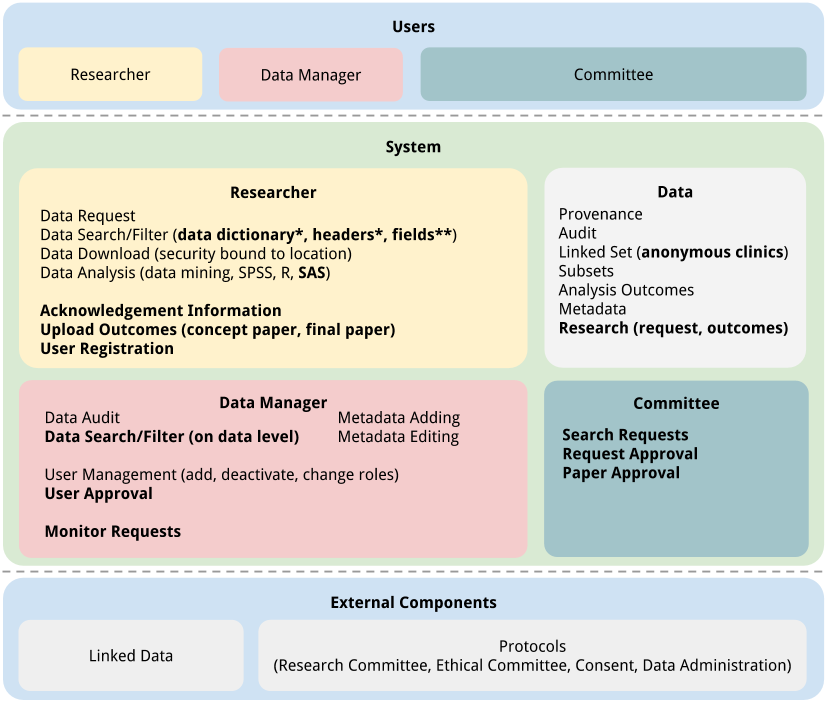
\includegraphics[width=1.0\linewidth]{images/brainstorm-after}
	\caption{
		\ivfsystem{} schema after brainstorm, encompassing data, user, request, and publication management.
		External services are provided and outside of the scope of this paper.
		Three direct users are planned each with their specific set of functions.
		Data listed is either available at initialisation of the system or is generated during execution.
		*: The data dictionary contains information about all the available data items, also called: headers.
		**: Fields are the raw (medical) data that belong to a stored pregnancy, fields are separated and named with headers.
	}
	\label{fig:brainstorm-after}
\end{figure}